\documentclass{article}
\usepackage[utf8]{inputenc}

\title{MS Azure Notes}
\author{Mark Potter}
\date{January 2021}

\usepackage{natbib}
\usepackage{graphicx}

\newcommand{\code}{\texttt}

\begin{document}

\maketitle

\begin{abstract}
This document serves as an accompaniment to the learning paths provided by Microsoft for working towards the AZ-204 exam. It may also be of interest to anyone looking for an overview of development on the Azure platform generally.
\end{abstract}

\section{Introduction}
These are notes I compiled while working through the learning paths for The Microsoft Azure Developer Certification AZ-204 in early 2021. I aim to keep the notes in line with the structure of the leaning paths at this time. 

\section{Create Serverless Apps}

This section lays out the serverless services offered by the Azure platform and walks you through creating Azure Functions. The learning path focuses predominately on using the Azure Portal to create functions however I opted to use Visual Studio Code (VSC) for most of the development. Instructions for setting up your development environment are covered by the learning path.

\subsection{Choose the best Azure service to automate your business processes}
Here we are introduced to four workflow implementation technologies:
\begin{itemize}
    \item Logic Apps
    \item Microsoft Power Automate
    \item WebJobs
    \item Azure Functions
\end{itemize}

they all \textbf{accept inputs}, \textbf{perform actions}, \textbf{support conditions} and \textbf{return outputs}.

These technologies fall into two categories: \textbf{design-first} technologies and \textbf{code first} technologies, with Logic Apps and MS Power Automate being design-first and WebJobs and Azure Functions being code-first. Design-first technologies let you create workflows with flow diagrams whereas code-first technologies require programming. 

\begin{figure}[h!]
\centering
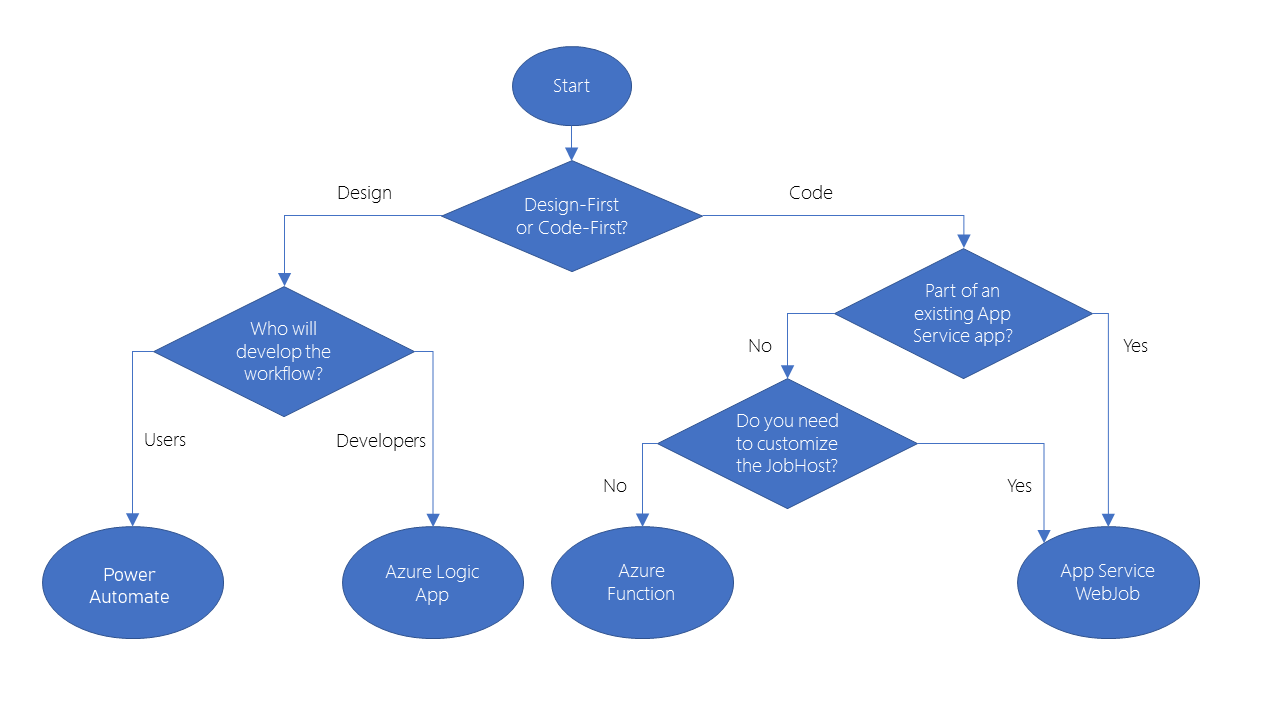
\includegraphics[scale=0.35]{service-choice-flow-diagram}
\caption{Decision tree for choosing a workflow implementation technology.}
\label{fig:service-choice-flow-diagram}
\end{figure}

\subsubsection{Logic Apps}
Logic apps can be created with either the flow diagram GUI or by writing your own JSON describing the workflow. Logic apps have \textbf{connector} components which let you interface with external services. There are over 200 builtin connectors and you can write your own. Logic apps are aimed at developers but are useful in situations where clear communication of what the workflow does is important to \textbf{non-technical} stakeholders. 

\subsubsection{Microsoft Power Automate}
MS Power Automate is similar to Logic Apps but is intended to be used by \textbf{non-technical} users. It works with a similar flow diagram style GUI but with no support for defining your own JSON. You can still create custom connectors and under the hood it's still just a Logic App.

\subsubsection{WebJobs}
WebJobs come in two flavours \textbf{continuous} and \textbf{triggered}. They can be written in a wide range of languages however the SDK only supports C\#. Using the SDK provides access to \code{JobHostConfiguration} and \code{HostBuilder} which let you interact the the Azure App Service 

\subsubsection{Azure Functions}
Azure functions only use resources when the function code is being run. They start in response to a \textbf{trigger}, all Azure functions have one. Example triggers are HTTP calls, timers or documents added to a database collection. You can create Azure Functions in the Azure Portal or in VSC. They should be your \textbf{default choice} when taking the code-first approach.

\subsection{Create serverless logic with Azure Functions}
Serverless compute is great because you don't have to manually provision infrastructure. You don't have to worry about over allocating resources as \textbf{instances are created and destroyed on demand}. However there are some instances in which Azure Functions may not be the best option. Azure Functions have a \textbf{maximum timeout of ten minutes} (two and half for functions invoked by HTTP). There's also a limit on scaling, you can only spawn \textbf{200 concurrent instances} of a function app and you can only \textbf{provision a new one every ten seconds}. \textit{N.B} One function app instance can service multiple requests so while there is no set limit to how much traffic an instance can handle it may be cheaper to host your service on a VM.

\subsubsection{Create a function app}
This section of the learning path walks you through creating a function app in the Azure Portal. You just need to fill in a few inputs in a form and the portal takes care of the rest. You'll get some example code which you can run and rewrite in the portal if you want to have a play. You can also make requests to the function's endpoint which you can reveal by clicking "Get function URL". cURL and Postman are good tools for this. You can also check the monitoring dashboard to see requests made to your function. This section also introduces the \code{context} object. Those using JavaScript will notice that in the default function code \code{context.log} is used where they might expect to see \code{console.log}. While \code{console.log} will not error in newer versions of the function app runtime it's use is discouraged because a \textbf{\code{console.log} will not be tied to a specific invocation of your function}. 

\subsubsection{Secure HTTP triggers}
When creating an HTTP triggered function you'll be asked to select an authorisation level. The Admin level will require your master key, the function level uses function keys which are scoped to this particular function, the anonymous level required no authorisation. To provide auth when making a request to your function you can either include your key with the query param \code{code} (\textit{eg} \code{https://my-app.azurewebsites.net/api/myFunc?code=<key>}) or by including an \code{x-functions-key} header with your request.   

%\bibliographystyle{plain}
%\bibliography{references}
\end{document}
